\documentclass[12pt,a4paper,oneside]{report}

\usepackage{fontspec}
\setmainfont{Times New Roman}
\setmonofont{Consolas}
\usepackage[top=2.2cm,bottom=2.2cm,left=3cm,right=2cm,headheight=15pt]{geometry}
\usepackage{graphicx}
\graphicspath{{images/}}
\usepackage{amsmath,amssymb}
\usepackage{booktabs,tabularx,array,longtable,multirow}
\usepackage{setspace}
\usepackage{xcolor}
\usepackage{listings}
\usepackage{float}
\usepackage{caption}
\usepackage{subcaption}
\usepackage{enumitem}
\usepackage{fancyhdr}
\usepackage{titlesec}
\usepackage{tikz}
\usetikzlibrary{arrows.meta,positioning,shapes.geometric,fit}
\usepackage{hyperref}

\definecolor{hcmusblue}{HTML}{173A7A}
\definecolor{accentblue}{HTML}{2867C7}
\definecolor{lightblue}{HTML}{EAF2FF}
\definecolor{lightgray}{HTML}{F4F6F8}
\definecolor{darkgray}{HTML}{374151}
\definecolor{goodgreen}{HTML}{207A4B}
\definecolor{warnorange}{HTML}{A45A00}

\hypersetup{
  colorlinks=true,
  linkcolor=hcmusblue,
  citecolor=hcmusblue,
  urlcolor=accentblue,
  pdftitle={Technical Report - Vietnamese Traffic Route Optimization},
  pdfauthor={Group 314}
}

\onehalfspacing
\setlength{\parindent}{1.1cm}
\setlength{\parskip}{3pt}
\setlength{\emergencystretch}{2em}
\raggedbottom
\setlist{noitemsep,topsep=4pt,leftmargin=1.4cm}

\titleformat{\chapter}[display]
  {\normalfont\bfseries\color{hcmusblue}}
  {\filleft\Large CHAPTER \thechapter}
  {0.4ex}{\titlerule[1.2pt]\vspace{1ex}\Huge}
\titlespacing*{\chapter}{0pt}{-18pt}{24pt}
\titleformat{\section}{\Large\bfseries\color{hcmusblue}}{\thesection}{0.7em}{}
\titleformat{\subsection}{\large\bfseries\color{darkgray}}{\thesubsection}{0.7em}{}

\pagestyle{fancy}
\fancyhf{}
\fancyhead[L]{\small Introduction to Artificial Intelligence - Lab 1}
\fancyhead[R]{\small Group 314}
\fancyfoot[C]{\thepage}
\renewcommand{\headrulewidth}{0.4pt}

\lstset{
  backgroundcolor=\color{lightgray},
  basicstyle=\ttfamily\small,
  keywordstyle=\color{accentblue}\bfseries,
  commentstyle=\color{goodgreen},
  stringstyle=\color{warnorange},
  numbers=left,
  numberstyle=\tiny\color{darkgray},
  numbersep=9pt,
  frame=single,
  rulecolor=\color{gray!45},
  breaklines=true,
  showstringspaces=false,
  tabsize=4
}

\newcommand{\completed}{\textcolor{goodgreen}{\textbf{Completed}}}
\newcommand{\partialstatus}{\textcolor{warnorange}{\textbf{Prototype / partial}}}
\newcommand{\code}[1]{\texttt{#1}}

\hbadness=10000

\begin{document}

% -----------------------------------------------------------------------------
% COVER PAGE - follows the supplied visual reference
% -----------------------------------------------------------------------------
\begin{titlepage}
\thispagestyle{empty}
\begin{center}
{\bfseries\large TRƯỜNG ĐẠI HỌC KHOA HỌC TỰ NHIÊN - ĐHQG TP.HCM}\\[-1pt]
{\bfseries\large KHOA CÔNG NGHỆ THÔNG TIN}\\[0.75cm]


\includegraphics[width=4.2cm]{hcmus-logo.png}\\[0.45cm]

{\large NHẬP MÔN TRÍ TUỆ NHÂN TẠO}\\[2pt]
{\large BÁO CÁO LAB 01}\\[0.75cm]

{\bfseries\LARGE VIETNAMESE TRAFFIC ROUTE}\\[2pt]
{\bfseries\LARGE OPTIMIZATION}\\[0.3cm]
{\large Search Algorithms on a Ho Chi Minh City Road Graph}

\vfill

\begin{tabular}{>{\bfseries}rl}
Giảng viên: & Bùi Tiến Lên \\
Giảng viên: & Bùi Duy Đăng \\
Giảng viên: & Võ Nhật Tân \\
\end{tabular}\\[0.18cm]
{\small ----------oOo----------}

\vfill

{\bfseries Sinh viên thực hiện}\\[0.2cm]
\begin{tabular}{p{7.2cm}r}
Dương Trung Hiếu & 24127040 \\
Nguyễn Hoàng Bảo Long & 24127201 \\
Trần Vũ Anh Kiệt & 24127196 \\
\end{tabular}

\vfill
{Thành phố Hồ Chí Minh, tháng 8 năm 2026}
\end{center}
\end{titlepage}

\pagenumbering{roman}

\chapter*{Abstract}
\addcontentsline{toc}{chapter}{Abstract}
This technical report describes a traffic route optimization application for a
directed road graph in Ho Chi Minh City. The canonical dataset contains 1,033
geographic vertices and 3,914 directed road segments.
Road segments store distance, nominal travel time, congestion, direction, road
type, and risk factors. The project implements DFS, BFS, UCS, Dijkstra, A*, and
Greedy Best-First Search for two-location routing, together with
Nearest-Neighbor and Held-Karp methods for multi-location routing. A FastAPI
backend exposes graph and search operations, while a React and Leaflet interface
displays the network and route controls.

Experiments on a reachable urban test case show that UCS, Dijkstra, and A*
produce the same minimum distance-mode cost. A* reduces expansions from 561 to
173 relative to UCS, while Greedy Best-First expands only 26 vertices but returns
a route whose cost is 40.9 percent higher. Held-Karp
reducing a five-location mixed-cost tour by 15.42 percent relative to the input
order. The FastAPI, React, visualization, and explanation flow is integrated.

\noindent\textbf{Keywords:} graph search, traffic routing, A*, Dijkstra,
multi-location optimization, FastAPI, React, Ho Chi Minh City.

\chapter*{Document Conformance}
\addcontentsline{toc}{chapter}{Document Conformance}
This report is organized directly from Section 4.9, ``Technical Report,'' of
the Lab 1 specification. Chapters 1 through 10 correspond to items (a) through
(j): group introduction, problem context, modeling, dataset, algorithm
principles, program flow, comparison, multi-location optimization, program
instructions, and limitations/future work. The assessment in Chapter 1 is based
on the final repository state inspected on August 18, 2026.

\tableofcontents
\listoffigures
\listoftables
\clearpage
\pagenumbering{arabic}

% -----------------------------------------------------------------------------
\chapter{Group Introduction}

\section{Group Information}
The project is prepared by Group 314 for Lab 1 of Introduction to Artificial
Intelligence. Table~\ref{tab:members} records the submitted member list.

\begin{table}[H]
\centering
\caption{Group members}
\label{tab:members}
\begin{tabular}{cll}
\toprule
\textbf{No.} & \textbf{Student} & \textbf{Student ID}\\
\midrule
1 & Dương Trung Hiếu & 24127040\\
2 & Nguyễn Hoàng Bảo Long & 24127201\\
3 & Trần Vũ Anh Kiệt & 24127196\\
\bottomrule
\end{tabular}
\end{table}

\section{Member Contributions}
Work was divided by technical area, with joint review of integration and the
final demonstration.

\begin{table}[H]
\centering
\caption{Specific contribution of each member}
\label{tab:contributions}
\small
\begin{tabularx}{\textwidth}{>{\raggedright\arraybackslash}p{4.1cm}X}
\toprule
\textbf{Member} & \textbf{Main contribution}\\
\midrule
Nguyễn Hoàng Bảo Long (Data \& Model) & Curated the road dataset, defined and validated the cost model, documented the data and modeling, and finalized the report and demo materials.\\
Trần Vũ Anh Kiệt (Core Algorithms) & Designed the graph structure; implemented BFS, DFS, UCS, A*, advanced and multi-location search; and optimized and debugged the algorithms.\\
Dương Trung Hiếu (Web/Local GUI) & Built the interface, map, route selection, traversal animations, route explanations and metrics, compared algorithms, and supported backend integration.\\
\bottomrule
\end{tabularx}
\end{table}

\section{Requirement Completion Level}
Table~\ref{tab:completion} summarizes the implemented and verified functions in
the final repository.

\begin{table}[H]
\centering
\caption{Completion status against the Lab 1 requirements}
\label{tab:completion}
\small
\begin{tabularx}{\textwidth}{p{4.4cm}p{3.1cm}X}
\toprule
\textbf{Requirement} & \textbf{Status} & \textbf{Evidence / remaining work}\\
\midrule
Vietnamese traffic graph and attributes & \completed & 1,033 nodes and 3,914 directed segments with distance, time, congestion, type, direction, and risks.\\
Two-location search & \completed & DFS, BFS, UCS, Dijkstra, A*, and Greedy return a common result model.\\
Traffic-aware cost and heuristics & \completed & Distance, time, and mixed modes plus Haversine heuristics.\\
Backend API & \completed & Graph information and route-search endpoints are implemented.\\
GUI and graph display & \completed & React/Leaflet loads \code{/api/graph}, supports map/dropdown selection, and draws the returned route.\\
Step-by-step visualization & \completed & Algorithm traces drive current, explored, frontier, candidate, and final-route states.\\
Multi-location routing & \completed & The GUI executes start--waypoint--destination legs; Nearest Neighbor and optimal Held-Karp are also implemented for visit-order optimization.\\
Route explanation & \completed & The backend derives congestion/risk summaries, optimality notes, and a Dijkstra reference comparison from the returned route.\\
Build and smoke verification & \completed & Backend imports the canonical graph and the production Vite build completes successfully.\\
\bottomrule
\end{tabularx}
\end{table}

% -----------------------------------------------------------------------------
\chapter{Problem Context}

\section{Selected Vietnamese Traffic Scenario}
The selected scenario is an educational urban navigation system for a subset of
Ho Chi Minh City. A user chooses a start intersection, a destination, optional
stops, a search algorithm, and an optimization objective. The system then
searches a directed street graph and visualizes the route.

Ho Chi Minh City traffic is an appropriate context because one-way roads,
variable congestion, narrow streets, construction, and flooding can make a
short route slower or less suitable than an alternative. Therefore, route
quality cannot be represented by physical distance alone.

\section{Real-World Problem}
For a two-location query, the system must return a valid directed path whose
objective cost is minimized or approximated by the chosen algorithm. For a
multi-location query, it must decide both the visiting order and the detailed
road path between consecutive stops. Users also need an explanation: whether
the route is shortest by distance, fastest by adjusted time, or best under the
combined cost.

\section{Why Optimization Is Useful}
Traffic-aware routing can reduce travel time, avoid risky segments, and make
algorithm behavior understandable. The project is also an instructional tool:
the explored-node sequence shows why uninformed and heuristic searches behave
differently on the same road network.

% -----------------------------------------------------------------------------
\chapter{Problem Modeling}

\section{State-Space Formulation}
The road network is a directed weighted graph $G=(V,E)$:
\begin{itemize}
\item A \textbf{state} is the current vertex identifier.
\item The \textbf{initial state} is the selected start vertex $s$.
\item The \textbf{goal test} succeeds when the current identifier equals $t$.
\item A \textbf{transition} follows an outgoing edge in the adjacency list.
\item A one-way street creates one transition; a two-way street creates two.
\item A \textbf{solution} is an ordered sequence from $s$ to $t$ that respects direction.
\end{itemize}

\section{Nodes and Edges}
A node contains \code{node\_id}, \code{name}, latitude, longitude, and a type
such as intersection. An edge contains source, target, physical distance,
nominal time, congestion level 1--5, road type, direction, and a list of risks.
The adjacency-list design uses $O(|V|+|E|)$ memory.

\section{Traffic-Aware Cost Function}
Let $d(e)$ be physical distance, $t(e)$ nominal time, and $c(e)$ congestion.
The implementation defines
\begin{align}
d_{\mathrm{eff}}(e)&=d(e)[1+0.1(c(e)-1)],\\
t_{\mathrm{eff}}(e)&=t(e)m(c(e))+r(e),
\end{align}
where $m(c)$ is $1.0,1.3,1.8,2.4,$ or $3.5$. The risk term adds 300 seconds for
flooding, 120 for construction, 60 for a narrow road, and 45 for a complex
intersection. The selected edge cost is
\begin{equation}
C(e)=\begin{cases}
d_{\mathrm{eff}}(e),&\text{distance mode},\\
t_{\mathrm{eff}}(e),&\text{time mode},\\
\frac{d_{\mathrm{eff}}(e)+10t_{\mathrm{eff}}(e)}{2},&\text{mixed mode}.
\end{cases}
\label{eq:cost}
\end{equation}

Congestion therefore changes both effective distance preference and travel
time. Mixed mode converts one second into 10 metres of equivalent cost, a design
choice based on an assumed urban speed near 10 m/s. The value is useful for
ranking routes within mixed mode; it is not a monetary cost and must not be
compared numerically with the other modes.

\section{Assumptions}
All costs are non-negative. Traffic values are static during one search. GPS
coordinates are accurate enough for straight-line heuristics, while edge times,
congestion, and risks are simulated attributes rather than live measurements.
The system assumes the selected vertices belong to a reachable directed region.

% -----------------------------------------------------------------------------
\chapter{Dataset}

\section{Creation Method and Scale}
The project uses hybrid data: real street/intersection names and GPS coordinates
from a Ho Chi Minh City area, augmented with simulated traffic conditions. The
canonical JSON contains 1,033 nodes and 3,914 directed road segments. This
exceeds the minimum Lab 1 requirement of 20 nodes and 30 edges.

\section{Representative Locations}
The complete location list is stored in \code{data/hcm\_traffic\_data.json}. Representative
vertices used in experiments are shown below.

\begin{table}[H]
\centering
\caption{Representative locations from the dataset}
\label{tab:locations}
\small
\begin{tabularx}{\textwidth}{p{1.5cm}Xl}
\toprule
\textbf{ID} & \textbf{Location} & \textbf{Role in experiments}\\
\midrule
0 & Đường Hồng Bàng - Đường Đặng Thái Thân & Benchmark start and tour depot\\
880 & Ngô Gia Tự & Benchmark destination / required stop\\
127 & Hoà Hảo - Nguyễn Tri Phương & Required stop\\
500 & Trần Thiện Chánh - Đường 3 Tháng 2 & Required stop\\
750 & Đường Hồng Bàng - Đường Nguyễn Thị Nhỏ & Required stop\\
\bottomrule
\end{tabularx}
\end{table}

\section{Attribute Semantics}
Distance is stored in metres and nominal time in seconds. Congestion is an
integer from 1 (smooth) to 5 (gridlock). Direction is \code{one-way} or
\code{two-way}. Road type distinguishes local roads, avenues, and alleys. Risk
factors include flooding, construction, narrow roads, and complex intersections.

\section{Data Quality and Connectivity}
The directed structure means that arbitrary endpoint pairs may still produce a
no-path result. Experiments therefore use explicitly verified pairs. The data
is suitable for algorithm comparison but does not claim citywide map
coverage or real-time accuracy.

% -----------------------------------------------------------------------------
\chapter{Algorithm Principles}

\section{Common Search Representation}
Each frontier entry is a \code{SearchNode} with a vertex ID, parent, accumulated
cost $g$, heuristic $h$, priority $f$, and incoming edge. When the goal is found,
parent pointers reconstruct the route. All algorithms return a
\code{SearchResult} containing path, explored order, cost, distance, time, count,
and execution time.

\section{Uninformed Search}
\subsection{Depth-First Search}
DFS uses a stack and expands the most recently generated state. On a small
example $S\rightarrow\{A,B\}$, if $B$ is pushed last, DFS explores the branch
through $B$ first. It is complete on this finite graph with visited-state
checking, but it is not optimal by hops or cost and depends strongly on
adjacency order.

\subsection{Breadth-First Search}
BFS uses a queue and expands all depth-$k$ states before depth $k+1$. In the
same example it compares both one-edge branches before deeper states. It is
complete and optimal only for number of edges when each step has equal cost;
it does not minimize weighted traffic cost.

\subsection{Uniform-Cost Search}
UCS uses a min-heap ordered by $g(n)$, so the cheapest partial route is expanded
first. With non-negative edges it is complete (subject to a positive minimum
step cost) and optimal. A higher-hop route may be selected if its accumulated
traffic cost is lower.

\section{Additional Single-Route Algorithms}
\subsection{Dijkstra's Algorithm}
For a single target and non-negative edge costs, Dijkstra has the same expansion
rule as UCS. The project intentionally exposes it as a separate algorithm but
delegates to the UCS implementation. It is complete and optimal under the
current cost model.

\subsection{A* Search}
A* combines known and estimated cost:
\begin{equation}f(n)=g(n)+h(n).\end{equation}
It expands the lowest $f$. The heuristic is Haversine distance in distance mode,
distance divided by 16.67 m/s in time mode, and
\begin{equation}h_{mixed}(n)=d_H(n,t)+10d_H(n,t)/16.67\end{equation}
in mixed mode. Because straight-line travel and maximum-speed travel are lower
bounds, the intended heuristic is admissible. With the same lower-bound metric
on every transition it is also intended to be consistent. This preserves
optimality while often reducing expansions relative to UCS.

\subsection{Greedy Best-First Search}
Greedy Best-First orders the heap only by $h(n)$. It moves geographically toward
the goal and may explore very few vertices, but it ignores accumulated cost.
Therefore it is not optimal; the visited set makes it terminate on the finite
dataset, though a poor heuristic can produce a poor route.

\section{Multi-Location Methods}
Nearest Neighbor repeatedly chooses the cheapest unvisited destination and is
fast but approximate. Held-Karp dynamic programming stores the best path for
each subset/current-stop pair. It guarantees an optimal tour over the selected
stops when pairwise route costs are correct, at $O(n^2 2^n)$ time and
$O(n2^n)$ space.

% -----------------------------------------------------------------------------
\chapter{Program Flow}

\section{System Architecture}
\begin{figure}[H]
\centering
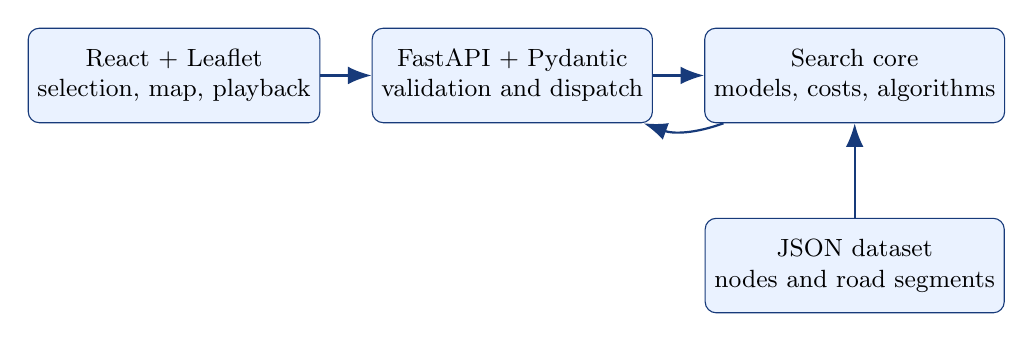
\begin{tikzpicture}[
  node distance=1.2cm,
  box/.style={draw=hcmusblue,rounded corners,fill=lightblue,minimum width=3.5cm,
    minimum height=1.2cm,align=center,font=\small},
  arrow/.style={-{Latex[length=3mm]},thick,color=hcmusblue}
]
\node[box] (ui) {React + Leaflet\\selection, map, playback};
\node[box,right=0.65cm of ui] (api) {FastAPI + Pydantic\\validation and dispatch};
\node[box,right=0.65cm of api] (ai) {Search core\\models, costs, algorithms};
\node[box,below=1.2cm of ai] (data) {JSON dataset\\nodes and road segments};
\draw[arrow] (ui) -- (api);
\draw[arrow] (api) -- (ai);
\draw[arrow] (data) -- (ai);
\draw[arrow,bend left=20] (ai) to (api);
\end{tikzpicture}
\caption{Three-layer system architecture}
\label{fig:architecture}
\end{figure}

\section{Main Processing Flow}
\begin{figure}[H]
\centering
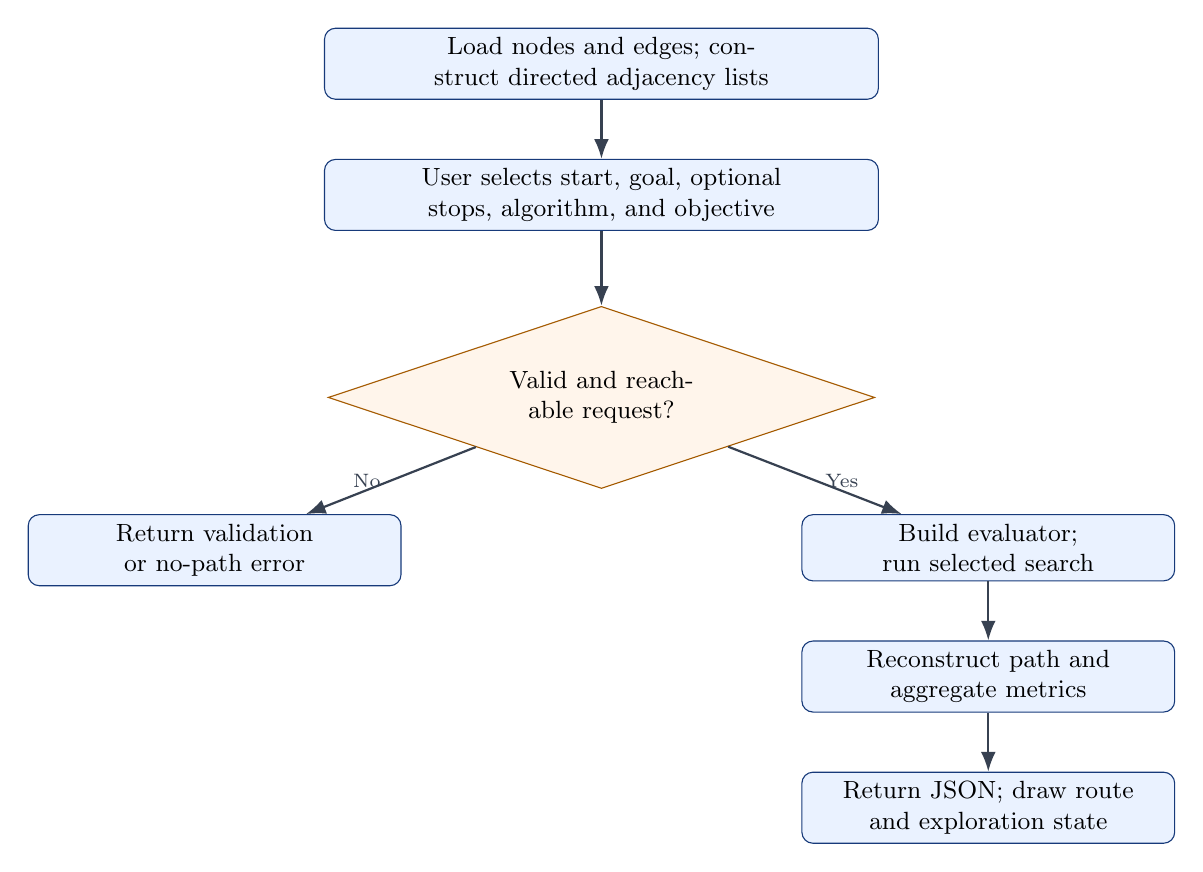
\begin{tikzpicture}[
  node distance=0.75cm,
  process/.style={draw=hcmusblue,rounded corners,fill=lightblue,
    text width=6.8cm,minimum height=0.8cm,align=center,font=\small},
  decision/.style={diamond,draw=warnorange,fill=orange!8,aspect=3,
    text width=4cm,align=center,font=\small},
  arrow/.style={-{Latex[length=2.5mm]},thick,color=darkgray}
]
\node[process] (load) {Load nodes and edges; construct directed adjacency lists};
\node[process,below=of load] (select) {User selects start, goal, optional stops, algorithm, and objective};
\node[decision,below=0.95cm of select] (valid) {Valid and reachable request?};
\node[process,text width=4.5cm,below left=0.9cm and 0.8cm of valid] (error) {Return validation or no-path error};
\node[process,text width=4.5cm,below right=0.9cm and 0.8cm of valid] (search) {Build evaluator; run selected search};
\node[process,text width=4.5cm,below=of search] (reconstruct) {Reconstruct path and aggregate metrics};
\node[process,text width=4.5cm,below=of reconstruct] (display) {Return JSON; draw route and exploration state};
\draw[arrow] (load) -- (select);
\draw[arrow] (select) -- (valid);
\draw[arrow] (valid) -- node[left,font=\scriptsize]{No} (error);
\draw[arrow] (valid) -- node[right,font=\scriptsize]{Yes} (search);
\draw[arrow] (search) -- (reconstruct);
\draw[arrow] (reconstruct) -- (display);
\end{tikzpicture}
\caption{Main route-search flow}
\label{fig:flow}
\end{figure}

\section{Modules and Responsibilities}
\begin{table}[H]
\centering
\caption{Program modules}
\label{tab:modules}
\small
\begin{tabularx}{\textwidth}{>{\raggedright\arraybackslash\ttfamily\footnotesize}p{5.3cm}X}
\toprule
\textbf{Module} & \textbf{Responsibility}\\
\midrule
src/models.py & Node/edge data classes, graph loader, risk and edge-cost calculation.\\
src/algorithms/base.py & Shared search-node/result types and path reconstruction.\\
src/algorithms/\newline bfs.py, dfs.py & Breadth-first and depth-first search with trace generation.\\
src/algorithms/\newline ucs.py, dijkstra.py & Non-negative weighted optimal search.\\
src/algorithms/\newline astar.py, greedy.py & Haversine-guided informed search.\\
src/algorithms/\newline multi\_location.py & Pairwise A* matrix, Nearest Neighbor, and Held-Karp.\\
backend/api.py & Graph endpoints, validation, algorithm dispatch, and response assembly.\\
frontend/src/ & Input controls, map, settings, route results, and playback controls.\\
\bottomrule
\end{tabularx}
\end{table}

\section{GUI Interaction}
The frontend imports graph data for immediate map display. A search request
sends start, end, algorithm, and optimization to FastAPI. The backend
selects a \code{CostEvaluator}, dispatches the algorithm, and returns path IDs,
coordinates, names, exploration order, metrics, trace steps, and an explanation.
The default API base is \code{/api}; Vite and Nginx proxy that prefix to FastAPI,
and backend alias normalization accepts both compact and display algorithm names.

% -----------------------------------------------------------------------------
\chapter{Algorithm Comparison}

\section{Theoretical Comparison}
\begin{table}[H]
\centering
\caption{Complexity, completeness, and optimality}
\label{tab:theory-comparison}
\small
\begin{tabularx}{\textwidth}{p{3.1cm}p{3.3cm}p{2.2cm}p{2cm}X}
\toprule
\textbf{Algorithm} & \textbf{Time} & \textbf{Memory} & \textbf{Complete} & \textbf{Optimal}\\
\midrule
DFS & $O(V+E)$ & $O(V)$ & Yes, finite graph & No\\
BFS & $O(V+E)$ & $O(V)$ & Yes & By hop count only\\
UCS & $O((V+E)\log V)$ & $O(V)$ & Yes & Yes, non-negative costs\\
Dijkstra & $O((V+E)\log V)$ & $O(V)$ & Yes & Yes, non-negative costs\\
A* & Exponential worst case & Exponential worst case & Yes under standard conditions & Yes with admissible/consistent $h$\\
Greedy Best-First & Exponential worst case & Exponential worst case & Yes on this finite implementation & No\\
Nearest Neighbor & $O(n^2)$ after cost matrix & $O(n)$ & Produces a tour if connected & No\\
Held-Karp & $O(n^2 2^n)$ & $O(n2^n)$ & Yes & Yes for selected stops\\
\bottomrule
\end{tabularx}
\end{table}

\section{Actual Two-Location Performance}
The verified query is vertex 0 (Đường Hồng Bàng - Đường Đặng Thái Thân) to
vertex 880 (Ngô Gia Tự) in distance mode. One local Python 3.13 run
produced Table~\ref{tab:actual}. Sub-millisecond differences are illustrative;
route quality and expansions are more meaningful on this small graph.

\begin{table}[H]
\centering
\caption{Actual distance-mode results from vertex 0 to 880}
\label{tab:actual}
\small
\begin{tabular}{lrrrrrr}
\toprule
\textbf{Method}&\textbf{Nodes}&\textbf{Dist. (m)}&\textbf{Time (s)}&
\textbf{Cost}&\textbf{Expanded}&\textbf{ms}\\
\midrule
DFS&340&36,329.18&35,533.10&43,507.72&512&86.215\\
BFS&18&2,430.24&1,567.80&2,782.52&590&38.883\\
UCS&26&1,978.48&2,039.70&2,149.45&561&41.674\\
Dijkstra&26&1,978.48&2,039.70&2,149.45&561&42.902\\
A*&26&1,978.48&2,039.70&2,149.45&173&8.171\\
Greedy Best-First&20&2,552.25&2,171.60&3,028.28&26&0.767\\
\bottomrule
\end{tabular}
\end{table}

UCS, Dijkstra, and A* agree on the optimum. A* reduces expansions by 69.2
percent relative to UCS. Greedy expands only 26 vertices but costs 40.9 percent
more than the optimum. BFS finds the fewest-edge route, not the cheapest route,
and DFS follows a long adjacency-order-dependent detour.

\section{Effect of Traffic Objective}
\begin{table}[H]
\centering
\caption{A* results under three optimization criteria}
\label{tab:objectives}
\begin{tabular}{lrrrrr}
\toprule
\textbf{Mode}&\textbf{Nodes}&\textbf{Dist. (m)}&\textbf{Time (s)}&
\textbf{Cost}&\textbf{Expanded}\\
\midrule
Distance&26&1,978.48&2,039.70&2,149.45&173\\
Time&18&2,248.98&1,185.60&1,185.60&369\\
Mixed&18&2,248.98&1,185.60&7,193.06&343\\
\bottomrule
\end{tabular}
\end{table}

Time mode accepts approximately 271 additional metres to reduce adjusted time
by 854.1 seconds (41.9 percent). This is direct evidence that congestion changes
the route. Mixed cost has a different unit, so only values within mixed mode are
comparable.

% -----------------------------------------------------------------------------
\chapter{Multi-Location Optimization}

\section{Problem Definition}
Given a depot and several required stops, the system must choose an order, find
the best road path between each consecutive pair, and return to the depot. The
pairwise cost matrix is intended to use A* with the selected evaluator. Nearest
Neighbor gives a fast approximate order; Held-Karp searches all subset states
and guarantees the best tour over the selected locations.

\section{Experimental Comparison}
The depot is vertex 0 and the supplied visit order is
$880\rightarrow127\rightarrow500\rightarrow750$. Mixed mode is used. Pairwise
road costs are computed directly by the current A* implementation.

\begin{table}[H]
\centering
\caption{Original and optimized multi-location orders}
\label{tab:tsp}
\small
\begin{tabularx}{\textwidth}{p{3.1cm}Xrr}
\toprule
\textbf{Method} & \textbf{Visiting order (including return)} &
\textbf{Path nodes} & \textbf{Mixed cost}\\
\midrule
Original input & 0 - 880 - 127 - 500 - 750 - 0 & -- & 40,753.249\\
Nearest Neighbor & 0 - 127 - 880 - 500 - 750 - 0 & -- & 36,806.586\\
Held-Karp DP & 0 - 500 - 880 - 127 - 750 - 0 & -- & 34,469.837\\
\bottomrule
\end{tabularx}
\end{table}

Held-Karp improves the original order by 15.42 percent and Nearest Neighbor by
6.35 percent. The remaining gap illustrates that locally cheapest decisions do
not guarantee the best cycle. Held-Karp is optimal for the five selected locations under the computed
pairwise mixed costs, but its exponential growth limits it to small stop sets.

\section{Integration Status}
The GUI supports user-specified waypoints by executing and joining consecutive
route-search legs, preserving per-leg traces, explanations, and aggregate
metrics. The separate Nearest Neighbor and Held-Karp routines optimize the
visiting order for small tours and reconstruct the complete road path.

% -----------------------------------------------------------------------------
\chapter{Program Instructions}

\section{Installation and Setup}
Prerequisites are Python 3.10 or later and Node.js 18 or later. From the project
root, install and run the backend:

\begin{lstlisting}[language=bash,caption={Backend setup}]
python -m pip install -r requirements.txt
python -m uvicorn backend.api:app --reload --port 8000
\end{lstlisting}

In a second terminal, run the frontend:
\begin{lstlisting}[language=bash,caption={Frontend setup}]
cd frontend
npm install
npm run dev
\end{lstlisting}

Open \url{http://localhost:5173}. Vite proxies \code{/api/*} requests to the
backend at \url{http://127.0.0.1:8000}. Alternatively, run the complete stack
with \code{docker compose up --build} and open \url{http://localhost:3000}.

\section{GUI Usage}
\begin{enumerate}
\item Select a start and destination by dropdown or map interaction.
\item Optionally add intermediate stops.
\item Choose Distance, Time, or Mixed optimization.
\item Choose DFS, BFS, UCS, Dijkstra, A*, or Greedy Best-First.
\item Press \textbf{Search}; inspect the path and route explanation panel.
\item Use the playback buttons to move through steps, then press Reset for a new query.
\end{enumerate}

\begin{figure}[H]
\centering
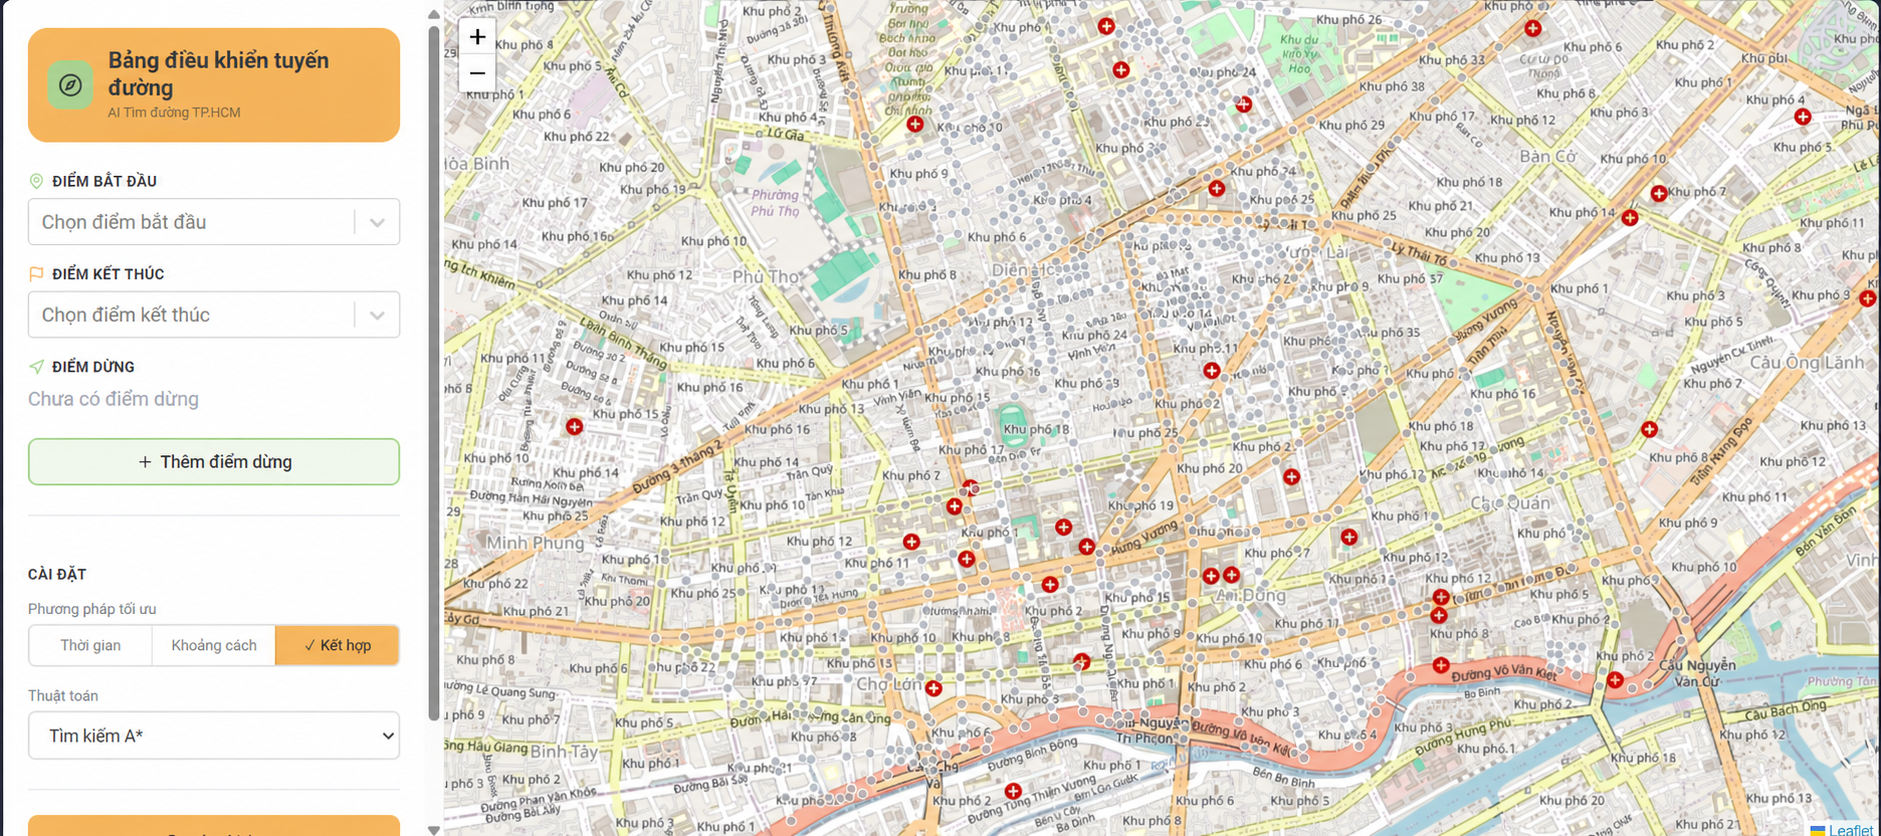
\includegraphics[width=0.9\textwidth]{system-interface.png}
\caption{React interface displaying the Ho Chi Minh City road graph}
\label{fig:gui}
\end{figure}

\section{Example Input and Output}
A direct backend request uses the schema below:

\begin{lstlisting}[language={},caption={Example search input}]
POST /api/search
{
  "start": "0",
  "end": "880",
  "algorithm": "astar",
  "optimization": "distance"
}
\end{lstlisting}

The response contains \code{algorithm\_name}, \code{path},
\code{explored\_nodes}, \code{total\_cost}, \code{total\_distance},
\code{total\_time}, \code{explored\_count}, \code{execution\_time\_ms}, names,
coordinates, trace \code{steps}, and a route explanation. For this example, A*
returns 26 path vertices, 1,978.48 metres, cost 2,149.45, and 173 expanded
vertices in the recorded run.

\section{Route Explanation Example}
The distance-mode A* route is selected because it has the lowest effective
distance cost among the tested weighted methods. BFS uses fewer road segments
but its cost is 29.5 percent higher. The time-mode alternative is physically
longer, yet its adjusted time is 854.1 seconds lower because it avoids more
costly traffic conditions. A* guarantees optimality only when its heuristic is
admissible/consistent; Greedy Best-First provides no such guarantee.

% -----------------------------------------------------------------------------
\chapter{Limitations and Future Work}

\section{Development Challenges}
The main challenges were transforming road data into a directed graph,
maintaining comparable metrics across algorithms, choosing traffic penalties,
and coordinating evolving backend/frontend interfaces. Directed connectivity
also makes a naive endpoint selection unreliable. Multi-location optimization
adds a second level of search because every pair of required stops needs a road
path before the visiting order can be optimized.

\section{Current Limitations}
\begin{itemize}
\item Traffic and risks are static simulated values rather than live observations.
\item The graph covers a limited urban area and contains vertices outside the largest strongly connected component.
\item Risk penalties and mixed-mode conversion are hand-designed, not statistically calibrated.
\item Reported route time is aggregated with a congestion formula that is not identical to every evaluator mode.
\item Waypoint legs use the user-supplied order in the GUI; automatic visit-order optimization remains a separate core routine.
\item Held-Karp has exponential growth and is suitable only for small stop sets.
\item The legacy standalone test runner targets an earlier module layout; broader API contract and regression coverage is needed.
\item Benchmarks use static snapshots and single local timings rather than repeated statistically summarized trials.
\end{itemize}

\section{Future Work}
The highest-priority work is to expose automatic visit-order optimization as a
dedicated API operation, replace the legacy runner with automated contract and
optimality tests, and add repeated performance benchmarks.

Longer-term extensions include real-time traffic feeds, map API integration,
time-dependent edge weights, alternative-route generation, turn restrictions,
bidirectional A*, support for multiple vehicles, and calibrated cost weights.
Experiments should repeat many reachable source-target pairs and report mean,
median, and variance instead of relying on one sub-millisecond run.

\section{Conclusion}
The repository provides a substantial classical-search foundation: a realistic
Vietnamese traffic graph, six single-route algorithms, traffic-aware objectives,
a REST service, and an interactive map. Reproducible results show the expected
optimality/efficiency trade-offs and demonstrate the value of optimizing beyond
distance. Held-Karp also provides a strong small-scale multi-location result.
The final FastAPI/React flow supports route selection, waypoint legs,
step-by-step visualization, aggregate metrics, and readable explanations.

% -----------------------------------------------------------------------------
\begin{thebibliography}{99}
\bibitem{lab1}
Introduction to Artificial Intelligence,
\textit{Lab 1: Search Algorithms for Vietnamese Traffic Route Optimization},
course specification, 2026.

\bibitem{russell2021}
Stuart Russell and Peter Norvig,
\textit{Artificial Intelligence: A Modern Approach}, 4th ed., Pearson, 2021.

\bibitem{hart1968}
Peter E. Hart, Nils J. Nilsson, and Bertram Raphael,
``A Formal Basis for the Heuristic Determination of Minimum Cost Paths,''
\textit{IEEE Transactions on Systems Science and Cybernetics}, 4(2), 1968.

\bibitem{cormen2022}
Thomas H. Cormen, Charles E. Leiserson, Ronald L. Rivest, and Clifford Stein,
\textit{Introduction to Algorithms}, 4th ed., MIT Press, 2022.

\bibitem{hcmusbrand}
University of Science, VNU-HCM,
\textit{HCMUS Brand Identity and Logo Usage Guide},
\url{https://hcmus.edu.vn/he-thong-nhan-dien-thuong-hieu/}, accessed August 18, 2026.

\bibitem{fastapi}
FastAPI, \textit{FastAPI Documentation},
\url{https://fastapi.tiangolo.com/}, accessed August 18, 2026.

\bibitem{react}
Meta Open Source, \textit{React Documentation},
\url{https://react.dev/}, accessed August 18, 2026.
\end{thebibliography}

\appendix
\chapter{Repository Structure}
\begin{verbatim}
data/hcm_traffic_data.json     Canonical road graph
src/models.py                  Graph and cost evaluator
src/algorithms/base.py         Common search types
src/algorithms/bfs.py          Breadth-first search
src/algorithms/dfs.py          Depth-first search
src/algorithms/ucs.py          Uniform-cost search
src/algorithms/dijkstra.py     Dijkstra search
src/algorithms/astar.py        A* search and heuristic
src/algorithms/greedy.py       Greedy Best-First search
src/algorithms/multi_location.py  Nearest Neighbor, Held-Karp
backend/api.py                 FastAPI endpoints
backend/schemas.py             Request/response schemas
frontend/src/                  React and Leaflet interface
\end{verbatim}

\chapter{Representative Optimal Route}
For the two-location distance experiment, UCS, Dijkstra, and A* return:
\begin{quote}\small
0 $\rightarrow$ 2 $\rightarrow$ 751 $\rightarrow$ 752 $\rightarrow$ 508
$\rightarrow$ 390 $\rightarrow$ 753 $\rightarrow$ 391 $\rightarrow$ 288
$\rightarrow$ 1016 $\rightarrow$ 966 $\rightarrow$ 849 $\rightarrow$ 841
$\rightarrow$ 43 $\rightarrow$ 33 $\rightarrow$ 31 $\rightarrow$ 46
$\rightarrow$ 824 $\rightarrow$ 825 $\rightarrow$ 879 $\rightarrow$ 41
$\rightarrow$ 885 $\rightarrow$ 39 $\rightarrow$ 881 $\rightarrow$ 882
$\rightarrow$ 880.
\end{quote}

\chapter{Requirement Traceability}
\begin{longtable}{p{2.1cm}p{5.2cm}p{5.5cm}}
\toprule
\textbf{Item} & \textbf{Required topic} & \textbf{Location in this report}\\
\midrule
\endhead
(a) & Group information, contributions, completion & Chapter 1\\
(b) & Problem context and usefulness & Chapter 2\\
(c) & Graph, state, transitions, attributes, cost & Chapter 3\\
(d) & Source, locations, values, assumptions & Chapter 4\\
(e) & Principles, examples, heuristic, guarantees & Chapter 5\\
(f) & Flowcharts, modules, GUI interaction & Chapter 6\\
(g) & Theory and actual algorithm comparison & Chapter 7\\
(h) & Multi-location method, orders, guarantee & Chapter 8\\
(i) & Setup, GUI use, examples, screenshot & Chapter 9\\
(j) & Challenges, limitations, extensions & Chapter 10\\
\bottomrule
\end{longtable}

\end{document}
